XML Encryption is a W3C standard used for encryption of XML documents~\cite{Eastlake2013}. It is typically used in Web Services applications or for encryption of SAML tokens in Single Sign-On scenarios.

XML Encryption defines (among others) two cryptographic algorithms: RSA PKCS\#1 v1.5 and AES/3DES in CBC (Cipher Block Chaining) mode of operation. These two algorithms are vulnerable to so called adaptive chosen-ciphertext attacks, which has been shown in many practical examples. Thus, it is not surprising that XML Encryption applications were also found to be vulnerable to those attacks:

\begin{itemize}
 \item In 2011, we presented a paper on How to Break XML Encryption~\cite{CCS:JagSom11}, which showed how to attack symmetric key encryption algorithms in CBC mode. The idea is very similar to the typical padding oracle attacks, it is just a slightly more complicated, since we use XML parsing errors as a side-channel. A very good summary on this attack gives Matthew Green.\footnote{\url{http://blog.cryptographyengineering.com/2011/10/attack-of-week-xml-encryption.html}}
 \item In 2012, we showed how to apply Bleichenbacher's attack on the asymmetric encryption algorithm (RSA PKCS#1) in XML Encryption~\cite{ESORICS:JagSchSom12}. A summary on Bleichenbacher's attack is given on our blog.\footnote{\url{http://web-in-security.blogspot.de/2014/08/old-attacks-on-new-tls-implementations.html}}
\end{itemize}

    
    

All you need to know for now is that both attacks belong to the family of adaptive chosen ciphertext attacks.

\begin{figure}[ht]
    \begin{center}
        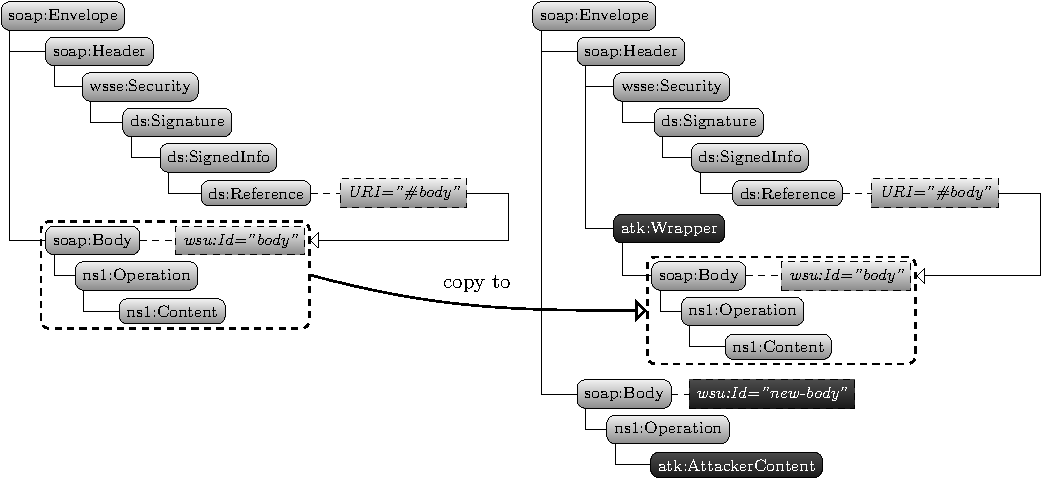
\includegraphics[width=\linewidth]{img/xsw_id}
    \end{center}
    \caption{Creating an XSW message for an ID referencing based XML Signature. 
The original signed message is shown on the left side.
The XSW message on the right side is constructed by copying the signed element to a \texttt{Wrapper} element and modifying the signed content to the attackers' needs.}
    \label{fig:xsw_id}
\end{figure}

The attacker, who eavesdrops an encrypted message, uses the message receiver as an oracle. He sends to the oracle modified ciphertexts and observes its response (it can contain a general error, a parsing failure, or just a valid response text). Based on the responses, he learns the plaintext.